\documentclass[aspectratio=169,11pt]{beamer}
\usetheme{Madrid}
\usepackage[T1]{fontenc}
\usepackage{lmodern}
\usepackage{amsmath,amssymb}
\usepackage{booktabs,tabularx,multicol}
\usepackage{tikz}
\usepackage{pgfplots}
\pgfplotsset{compat=1.17}
\usetikzlibrary{arrows.meta,positioning,fit,calc}

% ---------- colours (same palette as the Phase-1 decks) ----------
\definecolor{navy}{HTML}{1F3A5F}
\definecolor{accent}{HTML}{2A78D6}
\definecolor{warm}{HTML}{EB6834}
\definecolor{aqua}{HTML}{1BAF7A}
\definecolor{gold}{HTML}{EDA100}
\definecolor{soft}{HTML}{EEF3FA}
\definecolor{ink}{HTML}{333333}
\colorlet{frozen}{navy!25}
\colorlet{train}{warm}
\setbeamercolor{structure}{fg=navy}
\setbeamercolor{palette primary}{bg=navy,fg=white}
\setbeamercolor{palette secondary}{bg=navy!85!black,fg=white}
\setbeamercolor{palette tertiary}{bg=navy!70!black,fg=white}
\setbeamercolor{frametitle}{bg=navy,fg=white}
\setbeamercolor{title}{bg=navy,fg=white}
\setbeamercolor{block title}{bg=accent,fg=white}
\setbeamercolor{block body}{bg=soft,fg=ink}
\setbeamercolor{block title alerted}{bg=warm,fg=white}
\setbeamercolor{block body alerted}{bg=warm!8,fg=ink}
\setbeamercolor{block title example}{bg=aqua,fg=white}
\setbeamercolor{block body example}{bg=aqua!8,fg=ink}
\setbeamertemplate{navigation symbols}{}
\setbeamertemplate{itemize items}[circle]
\setbeamertemplate{section in toc}[sections numbered]

\newcommand{\code}[1]{\texttt{\small #1}}
\newcommand{\ent}[2]{\colorbox{#1!18}{\strut #2}}
\newcommand{\tg}[1]{{\scriptsize\color{warm}#1}}

% boxes for the adaptation diagrams
\tikzset{
  mat/.style={draw=navy, thick, minimum height=1.0cm, minimum width=1.0cm, fill=frozen, font=\small},
  lr/.style={draw=warm, thick, fill=warm!25, font=\small},
  vec/.style={draw=navy!60, fill=white, minimum width=0.5cm, minimum height=0.5cm, font=\small},
  arr/.style={-{Stealth[length=2mm]}, thick, navy},
}

\title[CS-781 Phase 2: Legal NER]{Phase 2: Legal Named Entity Recognition}
\subtitle{Six ways to adapt the Phase-1 legal LMs, explained with examples}
\author[Manish Kumar]{Manish Kumar (251330604)}
\institute{CS-781, IIT Kanpur}
\date{October 2026}

\begin{document}

\begin{frame}
  \titlepage
\end{frame}

\begin{frame}{Outline}
  \begin{multicols}{2}
  \tableofcontents
  \end{multicols}
\end{frame}

% =====================================================================
\section{The task}

\begin{frame}{L-NER: find the entity, its exact characters, and its legal role}
  \begin{columns}[T]
    \begin{column}{0.56\textwidth}
      \scriptsize
      \begin{exampleblock}{A real training document (fold1, id 115651329)}
        \ldots\ JAGE RAM \& ORS. ..Appellants Versus
        \ent{warm}{STATE OF HARYANA}\tg{RESP} ..Respondent
        \ldots\ the judgment dated \ent{aqua}{19.8.2011}\tg{DATE} passed by the
        \ent{accent}{High Court of Punjab and Haryana}\tg{COURT} in Criminal \ldots
      \end{exampleblock}
      \begin{block}{Required output (\code{prediction.json})}
        \code{\{"115651329": [[137, 153, "RESP"],}\\
        \code{\ \ \ \ \ \ \ \ \ \ \ \ \ \ \ \ [252, 261, "DATE"],}\\
        \code{\ \ \ \ \ \ \ \ \ \ \ \ \ \ \ \ [276, 308, "COURT"], ...]\}}
      \end{block}
      \begin{alertblock}{Strict scoring}
        Start, end \emph{and} label must all match:
        \code{[275, 308, "COURT"]} scores zero. Metric: macro-F1 over 12 labels.
      \end{alertblock}
    \end{column}
    \begin{column}{0.42\textwidth}
      \footnotesize
      \textbf{Data}
      \begin{itemize}
        \item Train: 70 judgments (fold1 + fold2), 8{,}393 entities.
        \item Test: 35 judgments (one is empty).
        \item $\approx$31k characters $\approx$6.6k tokens per document.
        \item No dev split: 10 training docs held out.
      \end{itemize}
      \textbf{Label counts (train)}\\[1mm]
      \begin{tabular}{@{}lr@{\hspace{4mm}}lr@{}}
        \toprule
        DATE & 1575 & APP & 407 \\
        PREC & 1183 & RESP & 381 \\
        STAT & 1260 & JUDGE & 245 \\
        COURT & 1013 & A.COUNSEL & 195 \\
        AUTH & 1003 & WIT & 187 \\
        CASENO & 760 & R.COUNSEL & 184 \\
        \bottomrule
      \end{tabular}\\[1mm]
      Macro-F1 weights rare R.COUNSEL equal to DATE: \textbf{class imbalance matters}.
    \end{column}
  \end{columns}
\end{frame}

% =====================================================================
\section{From characters to tags and back}

\begin{frame}{Step 1: tokens with character offsets}
  \begin{columns}[T]
    \begin{column}{0.5\textwidth}
      \footnotesize
      The Phase-1 byte-level BPE returns, for every token, the characters it covers.
      A token usually carries its leading space (\code{Ġ}), so we strip it:
      \vspace{1mm}

      \begin{tabular}{@{}llll@{}}
        \toprule
        token & raw offsets & stripped & text \\
        \midrule
        \code{Ġdated} & (245, 251) & (246, 251) & dated \\
        \code{Ġ19} & (251, 254) & (252, 254) & 19 \\
        \code{.} & (254, 255) & (254, 255) & . \\
        \code{8} & (255, 256) & (255, 256) & 8 \\
        \code{.} & (256, 257) & (256, 257) & . \\
        \code{2011} & (257, 261) & (257, 261) & 2011 \\
        \bottomrule
      \end{tabular}

      \vspace{2mm}
      Entity \code{[252, 261, DATE]} = first token start \ldots\ last token end.
    \end{column}
    \begin{column}{0.48\textwidth}
      \footnotesize
      \begin{alertblock}{Problem: punctuation runs are merged}
        BPE: \code{(AIR 1990 SC 79).} $\to$ \code{( AIR Ġ1990 ĠSC Ġ79 ).}\\
        The precedent ends after \code{)} but the token is \code{).}
        $\Rightarrow$ no tagger can output the right end.
      \end{alertblock}
      \begin{exampleblock}{Fix: \code{data.presplit: true}}
        Split words / digits / single punctuation \emph{before} BPE:
        \code{( AIR Ġ1990 ĠSC Ġ79 ) .}\ Words stay intact.
      \end{exampleblock}
      \begin{tabular}{@{}lcc@{}}
        \toprule
        & tokens & oracle macro-F1 \\
        \midrule
        plain BPE & 458{,}158 & 0.9866 \\
        presplit & 465{,}081 & \textbf{0.9945} \\
        \bottomrule
      \end{tabular}\\[1mm]
      {\scriptsize Oracle: gold $\to$ tags $\to$ spans, the pipeline's ceiling.}
    \end{column}
  \end{columns}
\end{frame}

\begin{frame}{Step 2: BIO tags, one per token (25 classes)}
  \footnotesize
  \begin{center}
  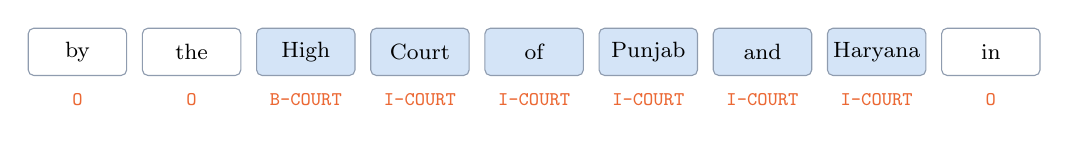
\begin{tikzpicture}[tok/.style={draw=navy!50, rounded corners=2pt, minimum height=6mm, inner sep=2pt, font=\footnotesize}]
    \foreach \w/\t/\c [count=\i] in {by/O/white, the/O/white, High/B-COURT/accent!20, Court/I-COURT/accent!20,
        of/I-COURT/accent!20, Punjab/I-COURT/accent!20, and/I-COURT/accent!20, Haryana/I-COURT/accent!20, in/O/white} {
      \node[tok, fill=\c, minimum width=1.25cm] (t\i) at (1.45*\i, 0) {\w};
      \node[font=\scriptsize\ttfamily, color=warm] at (1.45*\i, -0.6) {\t};
    }
  \end{tikzpicture}
  \end{center}
  \begin{columns}[T]
    \begin{column}{0.48\textwidth}
      \begin{block}{Encoding (training)}
        \begin{itemize}
          \item Tags: \code{O} + \code{B-X}, \code{I-X} for 12 labels = 25.
          \item A token gets the entity's tag if its visible characters overlap the span.
          \item First token \code{B-}, the rest \code{I-}.
        \end{itemize}
      \end{block}
    \end{column}
    \begin{column}{0.48\textwidth}
      \begin{block}{Decoding (prediction)}
        \begin{itemize}
          \item Run of \code{B-X I-X \ldots} $\to$ one span \code{[start(first), end(last), X]}.
          \item Trailing whitespace trimmed.
          \item Alternative design (not used yet): span classification / start--end pointers.
        \end{itemize}
      \end{block}
    \end{column}
  \end{columns}
\end{frame}

\begin{frame}{Step 3: long documents, 512-token windows}
  \begin{columns}[T]
    \begin{column}{0.52\textwidth}
      \footnotesize
      A document ($\approx$6.6k tokens) is longer than the window, so it is cut into overlapping windows.
      \begin{center}
      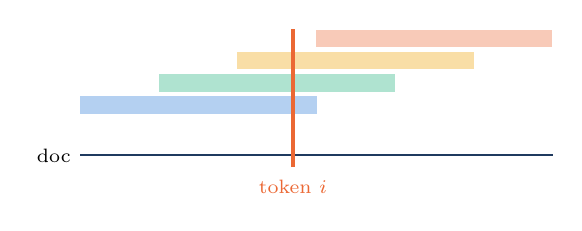
\begin{tikzpicture}[x=0.75cm]
        \draw[thick, navy] (0,0) -- (8,0);
        \node[font=\scriptsize, left] at (0,0) {doc};
        \foreach \s/\c [count=\i] in {0/accent, 1/aqua, 2/gold, 3/warm} {
          \fill[\c!35] (\s*1.33, 0.25+0.28*\i) rectangle ++(4, 0.22);
        }
        \draw[warm, very thick] (3.6, -0.15) -- (3.6, 1.6);
        \node[font=\scriptsize, warm] at (3.6, -0.4) {token $i$};
      \end{tikzpicture}
      \end{center}
      \textbf{Training}: window 512, stride 256, a random shift each epoch so entities land at new positions.

      \textbf{Inference}: stride 128. Token $i$ is covered by several windows; it keeps the
      logits of the one where it has the \emph{most context}:
      \begin{itemize}
        \item bidirectional model: $\max \min(\text{left}, \text{right})$ (most central),
        \item causal model: $\max$ left context.
      \end{itemize}
    \end{column}
    \begin{column}{0.46\textwidth}
      \footnotesize
      \begin{exampleblock}{Example}
        Token 700, stride 128, window 512.\\
        Windows starting at 256, 384, 512, 640 cover it.\\
        Left / right context: 444/67, 316/195, 188/323, 60/451.\\
        Bidirectional pick: start 384 ($\min = 195$).\\
        Causal pick: start 256 (444 tokens on the left).
      \end{exampleblock}
      \begin{block}{Why this matters}
        Parties (APP/RESP) are decided by cues like \emph{``..Appellants Versus''} which can
        sit in another window. Window size and stride are tuning knobs (later slide).
      \end{block}
    \end{column}
  \end{columns}
\end{frame}

\begin{frame}{Step 4: Viterbi decoding keeps the BIO sequence valid}
  \begin{columns}[T]
    \begin{column}{0.5\textwidth}
      \footnotesize
      Argmax per token can produce impossible sequences (illustration):
      \begin{center}
      \begin{tabular}{@{}lccc@{}}
        \toprule
        token & \code{Kashiram} & \code{\&} & \code{Ors} \\
        \midrule
        argmax & \code{O} & \code{I-PREC} & \code{I-PREC} \\
        Viterbi & \code{O} & \code{O} & \code{O}\\
        \ \ or & \code{B-PREC} & \code{I-PREC} & \code{I-PREC} \\
        \bottomrule
      \end{tabular}
      \end{center}
      Viterbi finds the most probable sequence that obeys:
      \begin{itemize}
        \item \code{I-X} only after \code{B-X} or \code{I-X},
        \item a document cannot start with \code{I-X}.
      \end{itemize}
      $$\hat y = \arg\max_{y\ \text{valid}} \sum_t \log p(y_t \mid x)$$
      Cost: $O(T \cdot 25^2)$, a few ms per document.
    \end{column}
    \begin{column}{0.46\textwidth}
      \footnotesize
      \begin{block}{Which one does it choose?}
        Whichever has the higher total log-probability:
        if \code{Kashiram} had $p(\text{B-PREC}) = 0.3$, \code{O}$=0.6$ and
        the \code{I-PREC} tokens are confident, the span version wins.
      \end{block}
      \begin{block}{Strict metric reminder}
        For every label $X$:
        $P_X = \frac{TP}{TP+FP}$, $R_X = \frac{TP}{TP+FN}$,
        $F1_X = \frac{2P_XR_X}{P_X+R_X}$.\\
        Macro-F1 = mean over the 12 labels.\\
        We also log \emph{span-only F1} (boundaries right, label ignored) to separate
        boundary errors from label confusion.
      \end{block}
    \end{column}
  \end{columns}
\end{frame}

\begin{frame}{Step 5: turning each Phase-1 model into a token encoder}
  \footnotesize
  \begin{tabularx}{\textwidth}{@{}l>{\raggedright\arraybackslash}X>{\raggedright\arraybackslash}X@{}}
    \toprule
    Model & What we feed / read & Attention for tagging \\
    \midrule
    A1 GPT & token + learned positions $\to$ 8 blocks $\to$ LayerNorm & causal mask removed (\code{attention: bidirectional}); max 1024 tokens \\
    A2 enc--dec & encoder reads the window; \textbf{decoder re-reads it} while cross-attending; tag decoder states (BART-style) & encoder bidirectional, decoder causal + full memory \\
    A3 prefix-LM & whole window = the ``prompt'' prefix & fully bidirectional, as in Phase-1 prompt reading \\
    A4 efficient & RoPE + GQA; local layers see $\pm$256 tokens, every 3rd layer global & causal mask removed \\
    \bottomrule
  \end{tabularx}
  \vspace{2mm}

  On top: dropout 0.1 + \textbf{linear head} $d \to 25$. Loss: cross-entropy over tags.
  \vspace{1mm}
  \begin{alertblock}{A2 finding: the encoder alone is almost useless}
    Mean cosine between A2 \emph{encoder} token vectors = \textbf{0.92} (A3: 0.19): nearly the same vector for every token.
    Tagging encoder states: 0.11 (adapters), 0.13 (partial FT), 0.15 (full FT) dev macro-F1.
    Tagging \emph{decoder} states: \textbf{0.39}. In Phase 1 the A2 decoder did most of the language modelling.
  \end{alertblock}
\end{frame}

% =====================================================================
\section{The adaptation techniques}

\begin{frame}{Overview: what each technique trains}
  \footnotesize
  \begin{center}
  \resizebox{\textwidth}{!}{%
  \begin{tabular}{@{}llllrr@{}}
    \toprule
    Run & Phase-1 model & Technique & What is trained & Trainable & Checkpoint \\
    \midrule
    E1 & A3 prefix-LM & Full fine-tuning & everything & 81.30M (100\%) & 325 MB \\
    E2 & A4 efficient & \textbf{LoRMA+} & low-rank multiplicative factors & 2.23M (2.5\%) & 9 MB \\
    E3 & A1 GPT & LoRA & low-rank additive factors & 1.79M (2.1\%) & 7 MB \\
    E4 & A2 enc--dec & Houlsby adapters & bottleneck MLPs + LayerNorms & 2.04M (2.2\%) & 8 MB \\
    E5 & A4 efficient & Partial (layer-wise) & top 4 of 10 blocks & 25.19M (28.8\%) & 101 MB \\
    E6 & A3 (4 of 8 blocks) & \textbf{Distillation} & student, taught by E1 & 52.95M (100\%) & 212 MB \\
    \bottomrule
  \end{tabular}}
  \end{center}
  \vspace{2mm}
  \begin{itemize}
    \item The token-classification head ($\approx$19k params) is trained in every run.
    \item PEFT checkpoints store only the trained tensors: the Phase-1 weights are re-loaded and the small file is applied on top.
    \item Also implemented, not submitted: BitFit (\code{peft.method: bitfit}).
  \end{itemize}
\end{frame}

% ---------------------------------------------------------------------
\begin{frame}{Full fine-tuning (E1, A3 prefix-LM)}
  \begin{columns}[T]
    \begin{column}{0.5\textwidth}
      \footnotesize
      \textbf{Idea.} Start from Phase-1 weights $W_0$ and update every one:
      $$W \leftarrow W - \eta\, \nabla_W \mathcal{L}_{\text{CE}}$$
      \textbf{Example.} A3: 8 blocks, $d=768$, 81.3M parameters, all trainable.
      Two learning rates: backbone $10^{-4}$ (small, keeps Phase-1 knowledge),
      new head $10^{-3}$ (starts random). Warm-up 10\% then cosine decay.
      \vspace{1mm}

      \textbf{Pros:} most capacity; simplest.\\
      \textbf{Cons:} 325 MB copy per task; can overwrite Phase-1 knowledge;
      most optimizer memory (AdamW: 2 extra values per weight).
    \end{column}
    \begin{column}{0.48\textwidth}
      \footnotesize
      \begin{center}
      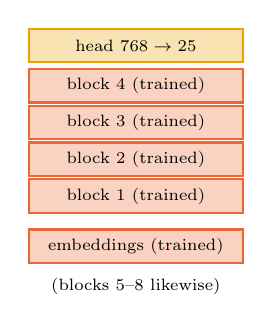
\begin{tikzpicture}[scale=0.85, transform shape, blk/.style={draw=warm, thick, fill=warm!30, minimum width=3.2cm, minimum height=5mm, font=\scriptsize}]
        \node[blk, fill=gold!30, draw=gold] (h) at (0,3.3) {head $768\to25$};
        \foreach \i in {1,...,4} \node[blk] (b\i) at (0, 0.55*\i+0.5) {block \i\ (trained)};
        \node[blk] (e) at (0,0.3) {embeddings (trained)};
        \node[font=\scriptsize] at (0,-0.3) {(blocks 5--8 likewise)};
      \end{tikzpicture}
      \end{center}
      \begin{exampleblock}{What we observed}
        Train loss $\to$ 0.0006; dev macro-F1 stays at 0.39--0.44 from epoch 6:
        it memorises the 60 training documents.
      \end{exampleblock}
    \end{column}
  \end{columns}
\end{frame}

% ---------------------------------------------------------------------
\begin{frame}{Partial / layer-wise fine-tuning (E5, A4 efficient)}
  \begin{columns}[T]
    \begin{column}{0.5\textwidth}
      \footnotesize
      \textbf{Idea.} Lower layers learn general features (spelling, syntax);
      upper layers are more task-specific. Freeze the bottom, train the top.
      \vspace{1mm}

      \textbf{Example.} A4 has 10 blocks. \code{n\_train\_layers: 4} trains blocks 7--10,
      the final RMSNorm and the head:
      $$\underbrace{4 \times 6.3\text{M}}_{\text{blocks}} + \text{norm} + \text{head} = 25.2\text{M} \;(28.8\%)$$
      Embeddings (24.6M) and blocks 1--6 stay frozen.
      \vspace{1mm}

      \textbf{Pros:} no gradients through frozen layers $\Rightarrow$ faster
      (96k tok/s vs 43k for E2) and less memory (2.3 GB).\\
      \textbf{Cons:} which layers to train is a guess; frozen features may be suboptimal.
    \end{column}
    \begin{column}{0.48\textwidth}
      \footnotesize
      \begin{center}
      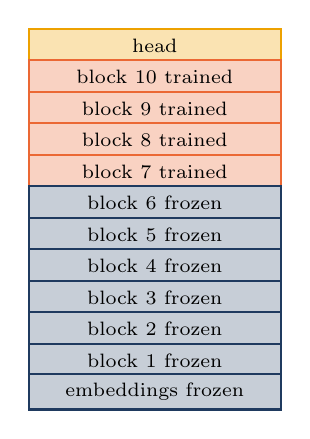
\begin{tikzpicture}[blk/.style={draw=navy, thick, minimum width=3.2cm, minimum height=4.2mm, font=\scriptsize}]
        \node[blk, fill=gold!30, draw=gold] at (0,4.0) {head};
        \foreach \i in {10,9,8,7} \node[blk, fill=warm!30, draw=warm] at (0, 0.4*\i - 0.4) {block \i\ trained};
        \foreach \i in {6,5,4,3,2,1} \node[blk, fill=frozen] at (0, 0.4*\i - 0.4) {block \i\ frozen};
        \node[blk, fill=frozen] at (0,-0.4) {embeddings frozen};
      \end{tikzpicture}
      \end{center}
      Result: 0.470 dev macro-F1, best epoch 6 (earliest of all runs).
    \end{column}
  \end{columns}
\end{frame}

% ---------------------------------------------------------------------
\begin{frame}{LoRA: low-rank \emph{additive} update (E3, A1 GPT)}
  \begin{columns}[T]
    \begin{column}{0.52\textwidth}
      \footnotesize
      \textbf{Idea} (Hu et al., 2022). The weight change needed for a new task has low rank.
      Keep $W_0$ frozen and learn $\Delta W = BA$:
      $$h = W_0 x + \frac{\alpha}{r}\, B A x, \qquad B\in\mathbb{R}^{d_{out}\times r},\ A\in\mathbb{R}^{r\times d_{in}}$$
      $B = 0$ at start $\Rightarrow$ the model begins exactly as the Phase-1 model.
      \vspace{1mm}

      \begin{exampleblock}{Parameter count for one A1 query matrix}
        $W_0$: $768\times768 = 589{,}824$ (frozen)\\
        $r=16$: $A$ $16\times768$ + $B$ $768\times16$ = \textbf{24{,}576} (4.2\%)\\
        Applied to q, k, v, o, fc, proj in 8 blocks: 1.77M + head = 1.79M.
      \end{exampleblock}
      $\alpha=32$, $r=16$ $\Rightarrow$ scale 2. Learning rate $10^{-3}$ (only small new matrices).
    \end{column}
    \begin{column}{0.46\textwidth}
      \begin{center}
      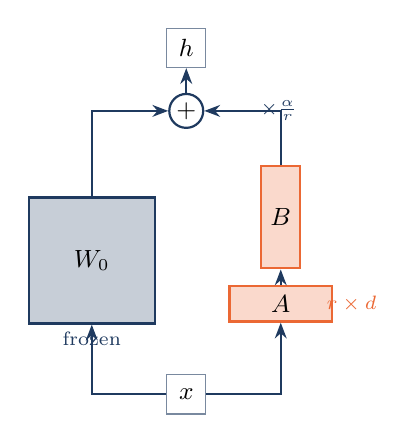
\begin{tikzpicture}[font=\small]
        \node[vec] (x) at (0,0) {$x$};
        \node[mat, minimum width=1.6cm, minimum height=1.6cm] (W) at (-1.2,1.7) {$W_0$};
        \node[lr, minimum width=1.3cm, minimum height=0.35cm] (A) at (1.2,1.15) {$A$};
        \node[lr, minimum width=0.35cm, minimum height=1.3cm] (B) at (1.2,2.25) {$B$};
        \node[circle, draw=navy, thick, inner sep=1pt] (p) at (0,3.6) {$+$};
        \node[vec] (h) at (0,4.4) {$h$};
        \draw[arr] (x) -| (W);
        \draw[arr] (x) -| (A);
        \draw[arr] (A) -- (B);
        \draw[arr] (W) |- (p);
        \draw[arr] (B) |- node[right, font=\scriptsize, pos=0.7] {$\times\frac{\alpha}{r}$} (p);
        \draw[arr] (p) -- (h);
        \node[font=\scriptsize, navy] at (-1.2,0.7) {frozen};
        \node[font=\scriptsize, warm] at (2.1,1.15) {$r\times d$};
      \end{tikzpicture}
      \end{center}
      \footnotesize
      Result: 0.356. Note A1 was trained \emph{causal}; we remove the mask, and
      LoRA's 2\% of parameters must adapt to that change too.
    \end{column}
  \end{columns}
\end{frame}

% ---------------------------------------------------------------------
\begin{frame}{LoRMA: low-rank \emph{multiplicative} update (E2, A4 efficient)}
  \begin{columns}[T]
    \begin{column}{0.54\textwidth}
      \scriptsize
      \textbf{Idea} (Bihany, Patel \& Modi, 2025). Instead of \emph{adding} a matrix,
      \emph{multiply} the frozen weight by a learned transformation:
      $$W = \Big(I + \tfrac{\alpha}{r} BA\Big) W_0,\quad B\in\mathbb{R}^{d_{out}\times r},\ A\in\mathbb{R}^{r\times d_{out}}$$
      \textbf{Rank inflation.} $BAW_0$ alone has rank $\le r$, too restrictive.
      Adding $I$ (\emph{LoRMA+}) makes the update full rank; with $B=0$ it starts at $W_0$.
      \vspace{1mm}

      \textbf{Reorder for speed} (never form $BAW_0$):
      $$h_0 = W_0x;\quad h = h_0 + \tfrac{\alpha}{r} B(A h_0)$$
      Same cost as LoRA. $A$ acts on the \emph{output} $h_0$, not on $x$.
      \begin{exampleblock}{A4 numbers ($r=16$; params $= 2 r\, d_{out}$)}
        \scriptsize q, o, proj: 24{,}576 each; k, v (GQA, 256 out): 8{,}192 each; gate, up (2048 out): 65{,}536 each.
        $\times$10 blocks + head = \textbf{2.23M} (2.5\%). Dev macro-F1 \textbf{0.486} (best run).
      \end{exampleblock}
    \end{column}
    \begin{column}{0.44\textwidth}
      \begin{center}
      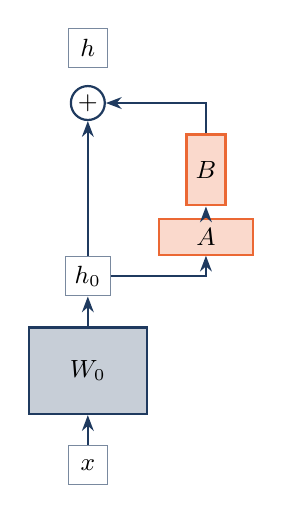
\begin{tikzpicture}[font=\small]
        \node[vec] (x) at (0,0) {$x$};
        \node[mat, minimum width=1.5cm, minimum height=1.1cm] (W) at (0,1.2) {$W_0$};
        \node[vec] (h0) at (0,2.4) {$h_0$};
        \node[lr, minimum width=1.2cm, minimum height=0.3cm] (A) at (1.5,2.9) {$A$};
        \node[lr, minimum width=0.3cm, minimum height=0.9cm] (B) at (1.5,3.75) {$B$};
        \node[circle, draw=navy, thick, inner sep=1pt] (p) at (0,4.6) {$+$};
        \node[vec] (h) at (0,5.3) {$h$};
        \draw[arr] (x) -- (W);
        \draw[arr] (W) -- (h0);
        \draw[arr] (h0) -- (p);
        \draw[arr] (h0) -| (A);
        \draw[arr] (A) -- (B);
        \draw[arr] (B) |- (p);
      \end{tikzpicture}
      \end{center}
    \end{column}
  \end{columns}
\end{frame}

\begin{frame}{LoRA vs LoRMA side by side}
  \footnotesize
  \begin{center}
  \begin{tabular}{@{}lll@{}}
    \toprule
    & LoRA & LoRMA+ \\
    \midrule
    Update & $W = W_0 + \frac{\alpha}{r}BA$ & $W = (I + \frac{\alpha}{r}BA)W_0$ \\
    $A$ shape & $r \times d_{in}$ (reads the input $x$) & $r \times d_{out}$ (reads the output $W_0x$) \\
    Rank of the change & $\le r$ & up to full ($BAW_0$ mixes all of $W_0$'s directions) \\
    Init & $A$ random, $B=0$ & $A$ random, $B=0$ \\
    Extra compute & $B(Ax)$ & $B(A\,W_0x)$, reusing $W_0x$ \\
    Params per $d\times d$ matrix & $2rd$ & $2rd$ \\
    Params when $d_{out}\ne d_{in}$ & $r(d_{in}+d_{out})$ & $2r\,d_{out}$ \\
    \bottomrule
  \end{tabular}
  \end{center}
  \begin{block}{Toy example, $d=2$, $r=1$}
    $W_0 = \begin{pmatrix}1&0\\0&2\end{pmatrix}$, $B = \begin{pmatrix}0.5\\0\end{pmatrix}$, $A = \begin{pmatrix}0&1\end{pmatrix}$, $\frac{\alpha}{r}=1$.\quad
    LoRA: $W = \begin{pmatrix}1&0.5\\0&2\end{pmatrix}$.\quad
    LoRMA+: $(I+BA)W_0 = \begin{pmatrix}1&0.5\\0&1\end{pmatrix}\begin{pmatrix}1&0\\0&2\end{pmatrix} = \begin{pmatrix}1&1\\0&2\end{pmatrix}$.\\
    LoRMA's update is \emph{scaled by what $W_0$ already does}: it re-combines existing output features.
  \end{block}
  {\scriptsize E2 vs E3 also differ in model (A4 vs A1): run LoRA on A4 to compare methods alone.}
\end{frame}

% ---------------------------------------------------------------------
\begin{frame}{Houlsby adapters (E4, A2 encoder--decoder)}
  \begin{columns}[T]
    \begin{column}{0.52\textwidth}
      \footnotesize
      \textbf{Idea} (Houlsby et al., 2019). Insert a small bottleneck MLP after a frozen sub-layer:
      $$y' = y + W_{up}\,\mathrm{GELU}(W_{down}\, y)$$
      $W_{down}: d\to m$, $W_{up}: m\to d$, $W_{up}=0$ at start (identity).
      Placed after \textbf{attention} and after the \textbf{MLP} of every block;
      LayerNorms are also trained.
      \vspace{1mm}

      \begin{exampleblock}{A2 numbers ($d=640$, $m=64$)}
        One adapter: $640\cdot64 + 64 + 64\cdot640 + 640 = 82{,}624$\\
        2 per block $\times$ 12 blocks (6 enc + 6 dec) = 1.98M\\
        + 32 LayerNorms (41k) + head (16k) = \textbf{2.04M} (2.2\%)
      \end{exampleblock}
      \textbf{vs LoRA:} adds sequential layers (slightly slower inference) but
      can apply a \emph{non-linear} correction.
    \end{column}
    \begin{column}{0.46\textwidth}
      \begin{center}
      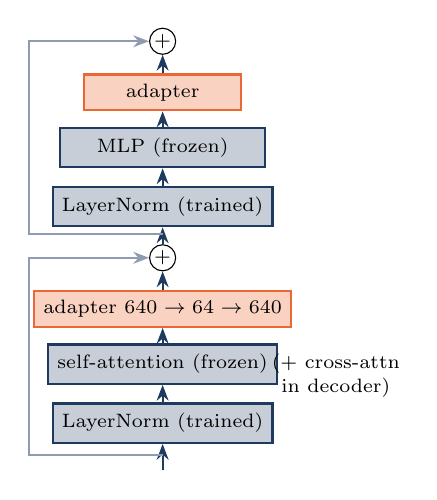
\begin{tikzpicture}[font=\scriptsize, sb/.style={draw=navy, thick, fill=frozen, minimum width=2.6cm, minimum height=5mm}, ad/.style={draw=warm, thick, fill=warm!30, minimum width=2.0cm, minimum height=4mm}]
        \node[sb] (ln1) at (0,0) {LayerNorm (trained)};
        \node[sb] (att) at (0,0.75) {self-attention (frozen)};
        \node[ad] (a1) at (0,1.45) {adapter $640\to64\to640$};
        \node[circle, draw, inner sep=0.5pt] (r1) at (0,2.1) {$+$};
        \node[sb] (ln2) at (0,2.75) {LayerNorm (trained)};
        \node[sb] (mlp) at (0,3.5) {MLP (frozen)};
        \node[ad] (a2) at (0,4.2) {adapter};
        \node[circle, draw, inner sep=0.5pt] (r2) at (0,4.85) {$+$};
        \foreach \a/\b in {ln1/att, att/a1, a1/r1, r1/ln2, ln2/mlp, mlp/a2, a2/r2} \draw[arr] (\a) -- (\b);
        \draw[arr] (0,-0.6) -- (ln1);
        \draw[arr, navy!50] (0,-0.4) -- (-1.7,-0.4) |- (r1);
        \draw[arr, navy!50] (0,2.4) -- (-1.7,2.4) |- (r2);
        \node[font=\scriptsize] at (2.2, 0.75) {(+ cross-attn};
        \node[font=\scriptsize] at (2.2, 0.45) {in decoder)};
      \end{tikzpicture}
      \end{center}
      \footnotesize
      Result: \textbf{0.389} with decoder states (0.112 on encoder states).
    \end{column}
  \end{columns}
\end{frame}

% ---------------------------------------------------------------------
\begin{frame}{BitFit (implemented, extra option)}
  \begin{columns}[T]
    \begin{column}{0.55\textwidth}
      \footnotesize
      \textbf{Idea} (Ben Zaken et al., 2022). Train only the bias vectors (and norm gains);
      every weight matrix stays frozen:
      $$h = W_0 x + \mathbf{b}, \qquad \text{only } \mathbf{b} \text{ is trained}$$
      \textbf{Example.} A3 block: biases of q,k,v,o (4$\times$768), fc (3072), proj (768),
      two LayerNorms (4$\times$768) $\approx$ 10.0k per block; 8 blocks + final norm + head
      = \textbf{100.6k}: \textbf{0.12\%} of the model.
      \vspace{1mm}

      \textbf{Caveat.} A4 uses bias-free linears and RMSNorm: BitFit on A4 trains only
      norm gains. Use it on A1, A2 or A3.
      \vspace{1mm}

      \code{python train.py --config configs/e1\_a3\_full.yaml}\\
      \code{\ \ --set peft.method=bitfit train.lr=1e-3 run\_name=E7\_a3\_bitfit}
    \end{column}
    \begin{column}{0.42\textwidth}
      \footnotesize
      \begin{block}{Where it sits}
        \begin{tabular}{@{}lr@{}}
          \toprule
          method & trainable \\
          \midrule
          BitFit (A3) & 0.12\% \\
          LoRA / LoRMA / adapters & 2--2.5\% \\
          Partial (top 4/10) & 29\% \\
          Full & 100\% \\
          \bottomrule
        \end{tabular}
      \end{block}
      A useful lower bound: how much can the Phase-1 features do with almost no change?
    \end{column}
  \end{columns}
\end{frame}

% ---------------------------------------------------------------------
\begin{frame}{Knowledge distillation (E6): teacher E1 $\to$ 4-block A3 student}
  \begin{columns}[T]
    \begin{column}{0.52\textwidth}
      \footnotesize
      \textbf{Idea} (Hinton et al., 2015). A small student imitates the full
      \emph{probability distribution} of a trained teacher, not only the gold tag:
      $$\mathcal{L} = \alpha\, \mathrm{CE}(y, p_s) + (1-\alpha)\, T^2\, \mathrm{KL}\big(p_t^{(T)} \,\|\, p_s^{(T)}\big)$$
      $p^{(T)} = \mathrm{softmax}(z/T)$. We use $\alpha = 0.5$, $T = 2$.
      $T^2$ keeps gradient sizes comparable as $T$ changes.
      \vspace{1mm}

      \textbf{Student init} (DistilBERT-style): keep Phase-1 A3 blocks 2, 4, 6, 8
      (\code{keep\_layers: [1,3,5,7]}), embeddings and final norm.
      \vspace{1mm}

      \begin{tabular}{@{}lrr@{}}
        \toprule
        & teacher E1 & student E6 \\
        \midrule
        blocks & 8 & 4 \\
        params & 81.3M & 52.9M \\
        tokens/s (train) & 91k & 130k \\
        dev macro-F1 & 0.439 & 0.344 \\
        \bottomrule
      \end{tabular}
    \end{column}
    \begin{column}{0.46\textwidth}
      \footnotesize
      \begin{exampleblock}{Why soften with $T$? A token's teacher logits}
        $z = (4, 2, 0)$ for (\code{B-COURT}, \code{B-AUTH}, \code{O})\\[1mm]
        $T=1$: $p = (0.87, 0.12, 0.02)$\\
        $T=2$: $p = (0.67, 0.24, 0.09)$\\[1mm]
        At $T=2$ the student also learns ``this looks a bit like an authority'':
        the \emph{dark knowledge} about which labels are confusable.
      \end{exampleblock}
      \begin{alertblock}{Params shrink less than blocks}
        Halving the blocks removes 28M, but the 24.6M embedding table stays.
        Smaller vocab / $d$ would compress further.
      \end{alertblock}
    \end{column}
  \end{columns}
\end{frame}

% =====================================================================
\section{Results}

\begin{frame}{Dev results (10 held-out documents, strict)}
  \begin{columns}[T]
    \begin{column}{0.55\textwidth}
      \scriptsize
      \begin{tabular}{@{}lrrrrr@{}}
        \toprule
        Run & macro-F1 & P & R & span-only & epoch \\
        \midrule
        E1 A3 full & 0.439 & 0.457 & 0.453 & 0.566 & 13 \\
        E2 A4 LoRMA & \textbf{0.486} & 0.518 & 0.478 & 0.573 & 13 \\
        E3 A1 LoRA & 0.356 & 0.395 & 0.356 & 0.503 & 15 \\
        E4 A2 adapter & 0.389 & 0.422 & 0.389 & 0.489 & 14 \\
        E5 A4 partial & 0.470 & 0.488 & 0.474 & 0.559 & 6 \\
        E6 A3 KD & 0.344 & 0.372 & 0.344 & 0.483 & 9 \\
        \bottomrule
      \end{tabular}
      \vspace{2mm}

      \begin{tabular}{@{}lrrr@{}}
        \toprule
        Run & train min & peak GPU & tok/s \\
        \midrule
        E1 & 2.1 & 3.7 GB & 91k \\
        E2 & 4.4 & 4.5 GB & 43k \\
        E3 & 2.8 & 3.2 GB & 67k \\
        E4 & 3.1 & 2.9 GB & 62k \\
        E5 & 1.4 & 2.3 GB & 96k \\
        E6 & 1.4 & 2.6 GB & 130k \\
        \bottomrule
      \end{tabular}
    \end{column}
    \begin{column}{0.43\textwidth}
      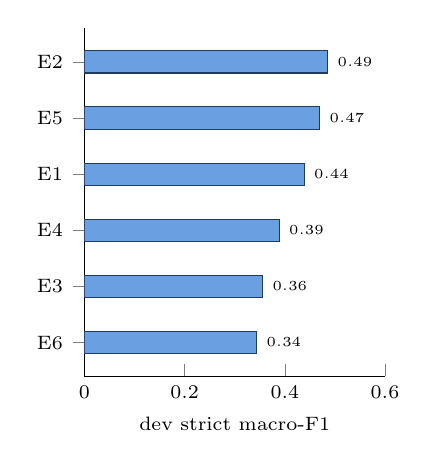
\begin{tikzpicture}
        \begin{axis}[xbar, width=5.4cm, height=6.0cm, xmin=0, xmax=0.6,
            symbolic y coords={E6,E3,E4,E1,E5,E2}, ytick=data, font=\scriptsize,
            nodes near coords, nodes near coords style={font=\tiny},
            xlabel={dev strict macro-F1}, bar width=8pt, enlarge y limits=0.12,
            axis x line*=bottom, axis y line*=left]
          \addplot[fill=accent!70, draw=navy] coordinates {(0.344,E6) (0.356,E3) (0.389,E4) (0.439,E1) (0.470,E5) (0.486,E2)};
        \end{axis}
      \end{tikzpicture}
      {\scriptsize Span-only F1 (boundary right, any label) is 0.08--0.13 above macro-F1:
      both boundaries \emph{and} labels lose points.}
    \end{column}
  \end{columns}
\end{frame}

\begin{frame}{Per-label dev F1: where the points are lost}
  \footnotesize
  \begin{center}
  \scriptsize
  \begin{tabular}{@{}lrrrrrrrrrrrr@{}}
    \toprule
    Run & APP & RESP & A.CO & R.CO & JUDGE & WIT & AUTH & COURT & STAT & PREC & DATE & CASENO \\
    \midrule
    E1 & .12 & .05 & .32 & .40 & .45 & .29 & .19 & .73 & .70 & .44 & .98 & .60 \\
    E2 & .12 & .06 & .62 & .67 & .47 & .21 & .20 & .79 & .67 & .40 & .98 & .64 \\
    E3 & .02 & .00 & .08 & .26 & .39 & .18 & .18 & .74 & .64 & .31 & .98 & .49 \\
    E4 & .06 & .11 & .42 & .48 & .27 & .17 & .16 & .76 & .60 & .28 & .95 & .42 \\
    E5 & .05 & .00 & .50 & .48 & .51 & .43 & .25 & .79 & .67 & .46 & .96 & .54 \\
    E6 & .08 & .00 & .17 & .18 & .41 & .21 & .22 & .74 & .66 & .23 & .92 & .32 \\
    \midrule
    dev gold & 114 & 93 & 20 & 31 & 33 & 44 & 226 & 97 & 165 & 232 & 190 & 60 \\
    \bottomrule
  \end{tabular}
  \end{center}
  \begin{columns}[T]
    \begin{column}{0.48\textwidth}
      \begin{block}{Example of an APP error (E1, test doc)}
        \scriptsize Text: \code{...HOUSING CO-OPEATIVE SOCIETY LTD.}
        E1 predicted \code{PAN} / \code{OPEATIVE} / \code{SOCIETY LTD}: three APP fragments.
        ALL-CAPS splits oddly: \code{ESSCO FABS} $\to$ \code{ES SCO ĠF AB S}.
      \end{block}
    \end{column}
    \begin{column}{0.48\textwidth}
      \begin{block}{Questions for the analysis}
        \scriptsize
        \begin{itemize}
          \item APP/RESP vs AUTH/COURT: label confusion or boundaries?
          \item How many errors sit in the document header?
          \item 20--44 gold A.COUNSEL / WIT: stable across seeds?
        \end{itemize}
      \end{block}
    \end{column}
  \end{columns}
\end{frame}

% =====================================================================
\section{Tuning points to try next}

\begin{frame}{Tuning points (1/3): data, context, imbalance}
  \footnotesize
  \begin{tabularx}{\textwidth}{@{}>{\raggedright\arraybackslash}p{3.3cm}>{\raggedright\arraybackslash}X>{\raggedright\arraybackslash}p{5.6cm}@{}}
    \toprule
    Knob & Why it may help & How to run \\
    \midrule
    Train on all 70 docs & +17\% data; keep the epoch count found on dev &
      \code{train.py ... --all-data --set train.epochs=13} \\
    Cross-validation on folds & 10 dev docs are noisy ($\pm$0.03); fold1$\leftrightarrow$fold2 gives 35-doc estimates &
      \code{--set data.split\_seed=1} (and a fold-split option) \\
    Longer window & party cues (``..Appellants Versus'') further away; A3/A4 have no length limit &
      \code{--set train.window=1024 infer.window=1024 train.batch\_size=8} \\
    Smaller inference stride & every token gets a more central window &
      \code{predict.py ... --set infer.stride=64} \\
    Down-weight \code{O} & 91\% of tokens are \code{O}; rare labels are recall-limited &
      \code{--set train.o\_weight=0.5} \\
    Per-label weights / focal loss & macro-F1 counts R.COUNSEL as much as DATE &
      new loss option: $w_X \propto 1/\sqrt{n_X}$ or $(1-p)^\gamma$ CE \\
    Case-normalise ALL-CAPS lines & \code{ESSCO FABS} $\to$ \code{Essco Fabs} tokenizes into familiar pieces; offsets unchanged (same length for ASCII) &
      preprocessing in \code{lner/data.py} before \code{tokenize} \\
    \bottomrule
  \end{tabularx}
\end{frame}

\begin{frame}{Tuning points (2/3): heads, decoding, post-processing}
  \footnotesize
  \begin{tabularx}{\textwidth}{@{}>{\raggedright\arraybackslash}p{3.3cm}>{\raggedright\arraybackslash}X>{\raggedright\arraybackslash}p{5.2cm}@{}}
    \toprule
    Knob & Why it may help & How to run \\
    \midrule
    MLP head & non-linear head over frozen PEFT features & \code{--set model.head=mlp} \\
    CRF layer & learns transition scores instead of hard Viterbi rules; a common gain in NER & new head: emissions + learned $25\times25$ transitions \\
    Span-based head & classify (start, end) pairs directly; fixes split entities like \code{PAN / OPEATIVE} & biaffine scorer over token pairs, max span length $\approx$40 tokens \\
    Argmax vs Viterbi & measure what the constraints buy & \code{predict.py --split dev --set infer.decode=argmax} \\
    Merge adjacent same-label spans & \code{SOCIETY} + \code{LTD} split by one token & post-process in \code{tags\_to\_spans} \\
    Document consistency & a party named once in the header recurs later with the same label & propagate high-confidence strings across the document \\
    Boundary trimming rules & trailing \code{.}, \code{,} or \code{)} wrongly included/excluded & compare predicted vs gold ends on dev, add rules \\
    \bottomrule
  \end{tabularx}
\end{frame}

\begin{frame}{Tuning points (3/3): adaptation and distillation}
  \footnotesize
  \begin{tabularx}{\textwidth}{@{}>{\raggedright\arraybackslash}p{3.0cm}>{\raggedright\arraybackslash}X>{\raggedright\arraybackslash}p{5.6cm}@{}}
    \toprule
    Knob & Why it may help & How to run \\
    \midrule
    Same method, other model & separates method effect from model effect (LoRA on A4, LoRMA on A1/A3) &
      e3 config \code{--set model.phase1\_ckpt=} \code{runs/A4\_efficient/best.pt} \\
    LoRA/LoRMA targets and rank & attention-only vs +MLP; $r \in \{4, 8, 32\}$ &
      \code{--set peft.targets=[q,v] peft.r=8} \\
    Causal vs bidirectional & does removing A1/A4's causal mask help or hurt? &
      \code{--set model.attention=causal} \\
    Layer-wise LR decay & full FT: smaller LR for lower layers protects Phase-1 features & optimizer groups per block, $\eta_l = \eta\,\xi^{L-l}$ \\
    Regularisation & E1 reaches loss 0.0006: overfitting & \code{--set model.dropout=0.2 train.weight\_decay=0.1} \\
    Fair KD baseline & same 4-block student \emph{without} the teacher shows the KD gain &
      \code{e6 config --set distill=null run\_name=E6\_noKD} \\
    Better teacher / KD knobs & E2 is stronger than E1; sweep $\alpha$, $T$; add hidden-state matching &
      \code{--set distill.alpha=0.3 distill.temperature=4} \\
    Further PEFT methods & extra submissions: prefix / prompt tuning, IA$^3$, LoRMA$_\pi$ & new \code{peft.method} entries \\
    \bottomrule
  \end{tabularx}
\end{frame}

\begin{frame}{Reproduce everything}
  \footnotesize
  \begin{block}{Commands (from \code{p2/})}
    \code{bash run\_all.sh} \hfill alignment check, E1--E6, six zips in \code{submissions/}\\
    \code{python train.py --config configs/e2\_a4\_lorma.yaml} \hfill one experiment\\
    \code{python predict.py --run runs/E2\_a4\_lorma} \hfill test zip\\
    \code{python predict.py --run runs/E2\_a4\_lorma --split dev} \hfill per-label dev report\\
    \code{python scripts/compare.py} \hfill \code{runs/comparison.md}
  \end{block}
  \begin{block}{Code map}
    \begin{tabular}{@{}ll@{}}
      \code{lner/data.py} & offsets, presplit, BIO encoding/decoding, windows \\
      \code{lner/backbones.py} & A1--A4 as token encoders, tagging head, KD student layers \\
      \code{lner/peft.py} & full, partial, BitFit, LoRA, LoRMA+, Houlsby adapters \\
      \code{lner/decoding.py} & argmax / Viterbi \\
      \code{lner/engine.py} & sliding-window inference, run loading \\
      \code{lner/metrics.py} & strict macro P/R/F1, span-only F1 \\
    \end{tabular}
  \end{block}
\end{frame}

\begin{frame}{References}
  \footnotesize
  \begin{itemize}
    \item H. Bihany, S. Patel, A. Modi. \emph{LoRMA: Low-Rank Multiplicative Adaptation for LLMs}. Findings of ACL 2025. arXiv:2506.07621.
    \item E. Hu et al. \emph{LoRA: Low-Rank Adaptation of Large Language Models}. ICLR 2022.
    \item N. Houlsby et al. \emph{Parameter-Efficient Transfer Learning for NLP}. ICML 2019.
    \item E. Ben Zaken, S. Ravfogel, Y. Goldberg. \emph{BitFit}. ACL 2022.
    \item G. Hinton, O. Vinyals, J. Dean. \emph{Distilling the Knowledge in a Neural Network}. 2015.
    \item V. Sanh et al. \emph{DistilBERT}. 2019.
    \item M. Lewis et al. \emph{BART}. ACL 2020 (decoder states for token classification).
    \item L. Ramshaw, M. Marcus. \emph{Text Chunking using Transformation-Based Learning} (BIO tags). 1995.
    \item J. Lafferty et al. \emph{Conditional Random Fields}. ICML 2001.
  \end{itemize}
\end{frame}

\end{document}
